\documentclass[../main.tex]
		
		\begin{document}
			\section{Forests and Trees}
	\begin{description}
		\item[Task:] Use the notion of a circuit to define trees.
		\item[Definition:] A graph is called acyclic if it contains no circuits (also known as cycles).
		\item[Definition:] A \underline{forest} is an acyclic graph.
		\item[Definition:] A \underline{tree} is a connected forest.
		\item[Examples:]
		\begin{enumerate}
			\item[]
			\item Is a tree and a forest.
			\begin{figure}[h!]
				\centering
				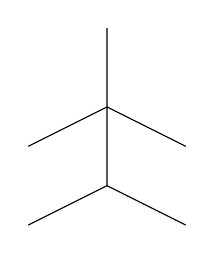
\begin{tikzpicture}
				\draw (0, 0) -- (0, -2) -- (-1, -2.5);
				\draw (-1, -1.5) -- (0, -1) -- (1, -1.5);
				\draw (0, -2) -- (1, -2.5); 
				\end{tikzpicture}
			\end{figure}
			\item Is a forest with 2 connected components (\textbf{i.e.} it consists of 2 trees.)
			\begin{figure}[h!]
				\centering
				\begin{tikzpicture}
				\coordinate (A) at (-3, 0);
				\coordinate (G) at (3, 0);
				\coordinate (C) at (-3, 1);
				\coordinate (H) at (3, 1);
				\coordinate (I) at (2.3, -0.7);
				\coordinate (J) at (3.7, -0.7);
				\coordinate (D) at (-3.7, 0.5);
				\coordinate (E) at (-3.6, -0.7);
				\coordinate (F) at (-2.3, -0.7);
				\coordinate (B) at (-2.3, 0.5);
				
				\draw (H) -- (G) -- (I);
				\draw (G) -- (J);
				
				\draw (D) -- (A) -- (C);
				\draw (B) -- (A) -- (F);
				\draw (A) -- (E);
				\end{tikzpicture}
			\end{figure}
		\end{enumerate}
		\item[Theorem:] Every forest contains at least one isolated or pendant vertex.
		\item[Proof:] Recall that when we studied circuits we proved a theorem that if $(V, E)$ is a graph s.t. $\forall v \in V$ deg $v \geq 2$ (\textbf{i.e.} $(V, E)$ has no isolated or pendant vertices), then $(V, E)$ contains at least one simple circuit. The graph $(V, E)$ is a forect, \textbf{i.e.} it contains no circuits $\Rightarrow \exists v \in V$ s.t. deg $v = 0$ or deg $v = 1$
		\item[qed]
		\item[Theorem:] A non-trivial tree contains at least one pendant vertex.
		\item[Proof:] A non-trivial tree $(V, E)$ must contain at least 2 vertices. Assum $\exists v \in V$ s.t. deg $v = 0$,\textbf{i.e.} $v$ is isolated, then $v$ forms a connected component by itself, but then $(V, E)$ has at least 2 connected components as $\#(V) \geq 2 \Rightarrow \Leftarrow$ to the fact that a tree is by definition connected. Therefore, $\forall v \in V,$ deg $v \geq 1$, but by the previous theorem $\exists v \in V$ s.t. $0 \leq$ deg $v \leq 1 \Rightarrow \exists v \in V$ s.t. deg $v = 1$ (since a tree is a forest).
		\item[qed]
		\item[Theorem:] Let $(V, E)$ be a tree, then $\# (E) = \# (V) - 1$, where $\#(E)$ is the number of edges of the tree and $\#(V)$ is the number of vertices.
		\item[Proof:] Use strong induction on $\#(V)$.
		\begin{description}
			\item[Base Case:] $\#(V) = 1$. The graph is trivial $\Rightarrow \#(E) = 0$, so $0 = 1-1$ as needed.
			\item[Inductive Step:] Suppose that every tree with $m$ vertices ($\# (V) = m$) has $m-1 = \#(v) -1 = \#(E)$ edges we seek to prove that if $(V, E)$ is a tree with $m+1$ vertices, then it has $m$ edges. \\
			By the previous theorem, $(V, E)$ has one pendent vertex. Let that vertex be $v$. Since deg $v = 1$, then there is only one edge incident to $v$. Let $vw$ be that edge. $w$ is then the only vertex of $(V, E)$ adjacent to $v$. We wish to reduce to the inductive hypothesis, the most natural way is to delete $w$ from $v$ and $vw$ from $E$. Let $V' = V \backslash \{v\}$ and $E' = E \backslash\{vw\} = \#(E) -1$. To use the inductive hyptohetsis, we must show $(V', E')$ is a tree, \textbf{i.e.} $(V', E')$ is connected and $(V' E')$ contains no circuits. $\forall v_1, v_2 \in V'$, since $(V, E)$ is a tree hence connected, $\exists$ path from $v_1$ to $v_2$ in $(V, E)$. This path cannot pass throgh $v$ because deg $v = 1 \Rightarrow$ is would have to pass through $v$ twice contradicting the fact that is it a path (all vertices are distinct) $\Rightarrow$ this path is in $(V', E') \Rightarrow (V' E')$ is connected. \\
			$(V', E')$ is a subgraph of $(V, E)$, which is a tree, hence does not containa ny circuits, so $(V', E')$ contains no circuits. \\
			$(V', E')$ is thus a tree, $\Rightarrow$ by the inductive hypothetsis, $\# (V') = \# (V) -1 = \# (E') - 1 = \# (E) -1 -1 = \#(E) - 2 \Rightarrow \#(V) -1 = \#(E) - 2 \Leftrightarrow \# (V) = \# (E)-1$ as needed.
			\item[qed]			
		\end{description}
	\end{description}

\end{document}
